% ===================================================
% CHAPITRE 8 — NAGU
% Pages imprimées 35-46 — vues 38-49
% ===================================================
\chapter{Nagu}

% --- Page imprimée 35 — vue 38
\begin{wrapfigure}{l}{0.40\textwidth}
    \vspace{-0.8\baselineskip}
    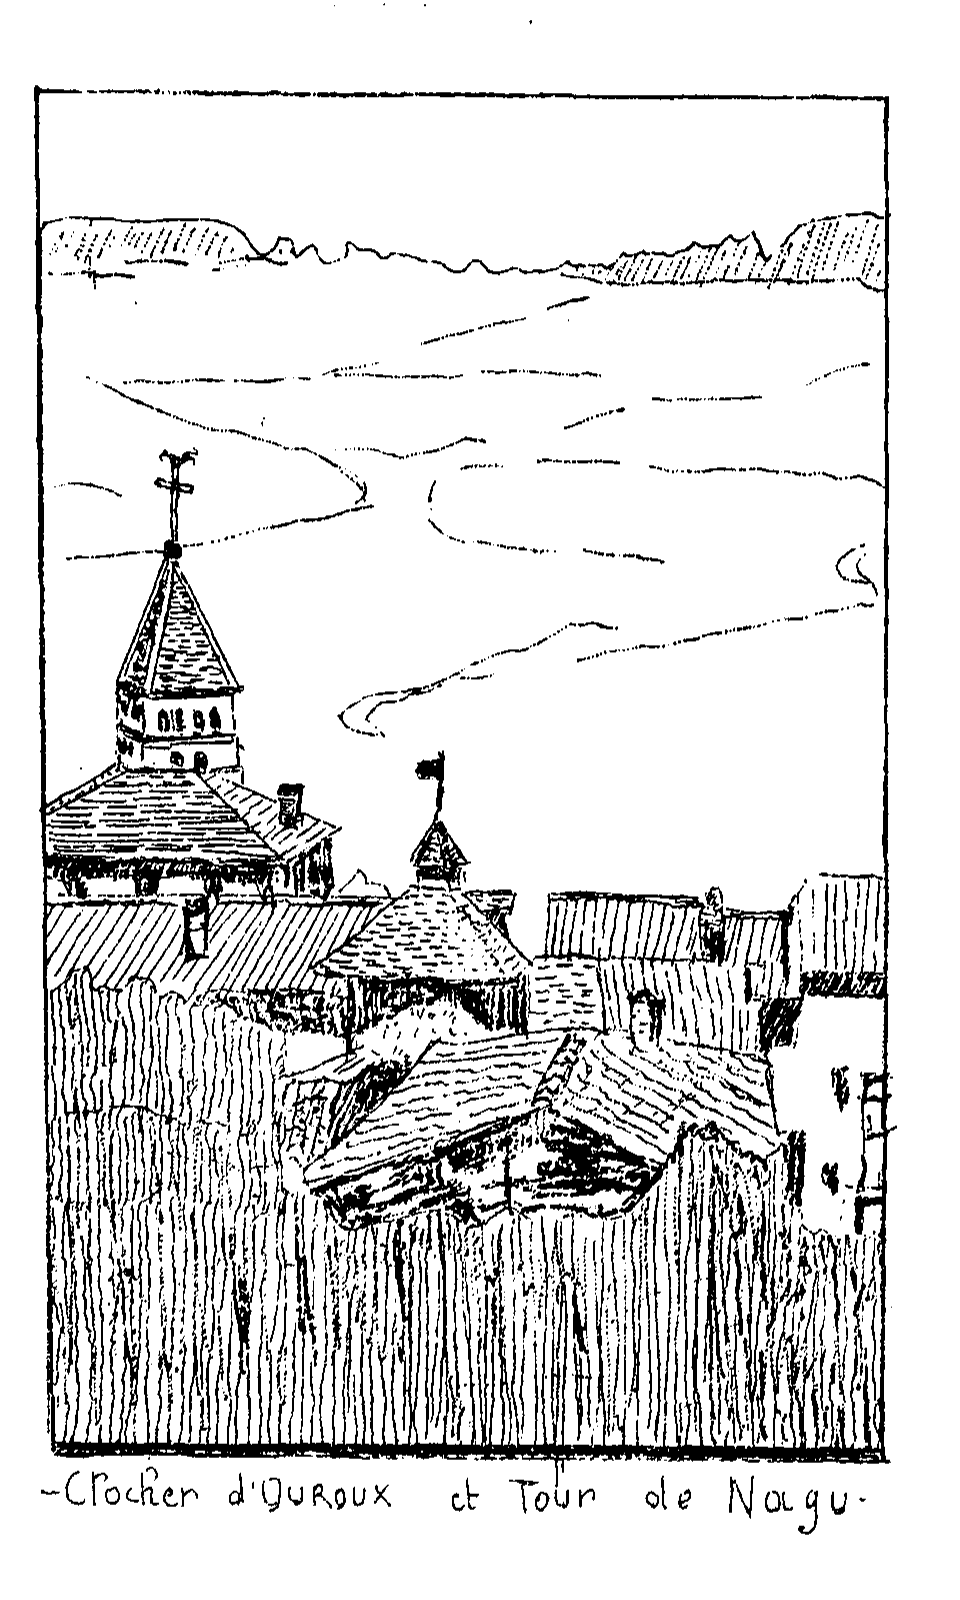
\includegraphics[width=0.38\textwidth]{Illustrations/illus-nagu-clocher-tour.png}
\end{wrapfigure}

Ce fief était situé dans le bourg même d'Ouroux. La tradition aussi bien que les documents nous le prouvent et la tour qui subsiste encore continue de porter le nom de cette puissante famille qui illustra dans les siècles passés, la noblesse du Beaujolais. Nagu fut le fief le plus important de cette paroisse et fut certainement érigé le premier.

Il nous serait impossible de déterminer à cette heure quels furent l'ensemble et l'étendue des constructions qui composèrent le château. Était-il construit au sommet du monticule qui domine le bourg? Nous serions portés à le croire, dans le principe du moins car là seulement il pouvait offrir des moyens de défense.

Les terres sur la ville présentaient alors, il y a quelques années, de nombreuses traces de construction ; ces vestiges ont dû disparaître successivement à la suite des travaux entrepris par les propriétaires. Nous avons vu nous-même mettre à découvert par suite du tracé d'un nouveau chemin de desserte, un fossé creusé dans le grès durci. Il offrait à la base une largeur de 1 m et de

% --- Page imprimée 36 — vue 39
2 m à sa partie supérieure, il avait environ 1 m de profondeur. Primitivement il devait être plus profond encore. Les dimensions étaient faciles à déterminer, la terre dont il avait été comblé étant une terre végétale tout à fait distincte du grès formant les parois. Ce fossé constituait-il une partie des défenses du château ? Nous ne saurions résoudre cette question. En tout cas les restes de murs devaient être plus récents et n'ont pu appartenir qu'au château de Nagu lui-même.

Le versant du monticule contre lequel s'est adossé le bourg offrait une disposition topographique toute différente de celle d'aujourd'hui. Il y a quatre ou cinq siècles, la montagne était à pic. À la suite d'un glissement considérable de terrain la pente fut moins prononcée et les propriétaires purent y établir des jardins. Ces jardins sont anciens car ils existaient, tels qu'ils sont à cette heure, au commencement du XVIe siècle. Un articulat Duligier en fait foi.

D'après Monsieur de Lacarelle, la tour qui existe encore faisait partie des travaux avancés destinés à défendre les approches de la place. Il faudrait alors admettre l'existence d'une seconde tour, disparue aujourd'hui et qu'une tradition très vague semble reporter au midi de celle qui existe. Elles eussent, dans ce cas, servi de défense à une porte donnant issue sur un chemin escarpé permettant de se rendre au château situé au sommet du monticule. C'est là une hypothèse que les fouilles faites jusqu'à présent ne permettent pas encore de vérifier.

Tout ce quartier a, du reste, subi de nombreuses modifications. De chaque côté de la tour de Nagu existaient des constructions assez vastes dont on connaît la direction générale. Les M.M. Gonnet, dans le but d'agrandir leur habitation, ont entrepris de déblayer une partie du terrain descendu de la montagne et dont nous parlions, plus haut. Ils ont mis à jour des murailles enfouies à plus de cinq mètres de profondeur et d'une solidité à toute épreuve.

À quelle époque remonte la tour de Nagu ? Étudions d'abord les divers éléments qui la composent. Sa base est rectangulaire, la partie du midi engagée récemment dans les bâtiments Gonnet a eu un de ses angles coupé afin d'augmenter les dimensions de l'appartement
% --- Page imprimée 37 — vue 40 (suite)
occupé. L'angle nord-ouest a été également abattu, dans ce siècle, pour permettre de construire un escalier qui donnât accès aux jardins.

Le rez-de-chaussée comprend un caveau voûté à plein cintre et n'ayant pour toute ouverture qu'un trou circulaire ménagé dans le centre de la calotte voûtée. Une porte basse, plus récente, mais dont les piliers paraissent anciens, y donne entrée. Les murs ont un mètre d'épaisseur.

\begin{wrapfigure}{r}{0.38\textwidth}
    \vspace{-0.5\baselineskip}
    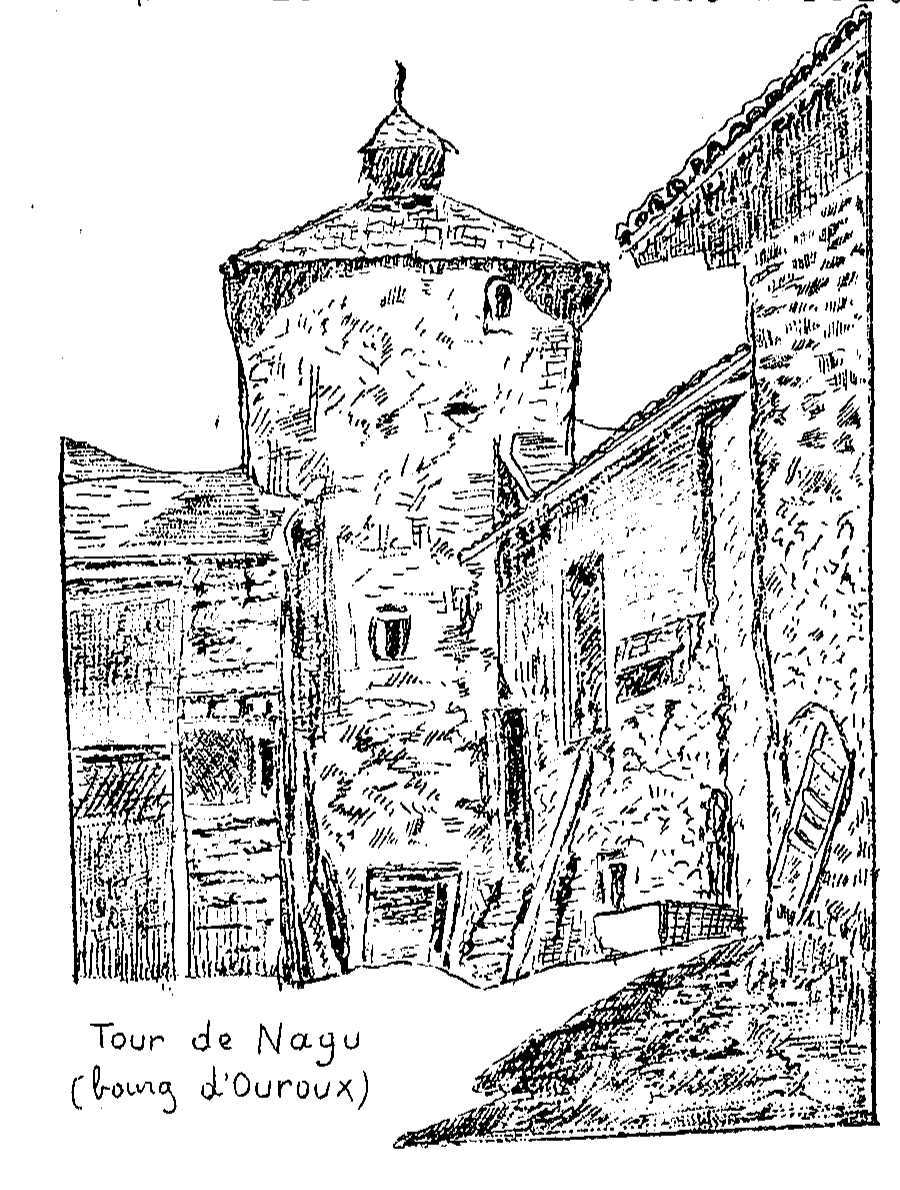
\includegraphics[width=0.35\textwidth]{Illustrations/illus-nagu-tour.png}
\end{wrapfigure}
Au premier étage, la tour prend insensiblement la forme circulaire pour la conserver tout-à-fait jusqu'au sommet. À l'intérieur ce premier étage est lui-même parfaitement circulaire, sauf dans le côté où se trouve la porte. La voûte est ogivale et présente une reproduction parfaite de celle de la coupole de l'église. Deux baies, très étroites et placées d'une manière fort irrégulière, donnent jour à cet étage. Étaient-elles destinées à servir de meurtrières ? C'est probable. L'une et l'autre étaient à tir rasant ; celle du midi était naguère encore à niveau des terres.

Enfin au deuxième étage une seule baie s'y voit encore. Si d'autres y étaient pratiquées, jadis, elles sont recouvertes par l'épais badigeon qui décore les murs.

Les nombreuses modifications que la toiture a dû subir ne permettent pas de déterminer quelle en était la disposition primitive.

La description que Monsieur Moretain a donnée de cette tour, description reproduite dans "La France par Cantons" est absolument incomplète. Cette tour, dit-il, servait à trois usages. Au milieu était une prison ; au bas, un noir cachot où l'on descendait la victime
% --- Page imprimée 38 — vue 41 (suite)
par une ouverture placée à la voûte ; le haut, maintenant démoli, était un appartement carré en dedans et en dehors et dont les angles faisaient saillie sur le rond de la tour.

Comme on le voit, Monsieur Moretain mentionne le rez-de-chaussée et le premier étage ; il passe sous silence le second qui n'a pas été modifié sauf en ce qui concerne la voûte qui devait être semblable à celle du premier étage. Quant à l'appartement carré dont il parle, le souvenir s'en est conservé jusqu'à nos jours. Le mode même de construction de ses murs nous porte à lui assigner une date plus récente. Ils étaient formés de briques encastrées dans des pièces de bois. Leur poids étant plus faible, il n'y avait aucune difficulté de faire porter leurs angles à faux en dehors de la tour elle-même. Peut-être ne devons-nous voir dans cette chambre qu'un simple colombier surajouté plus tard à la tour elle-même.

Voici d'ailleurs le sentiment qui nous paraît le plus probable au sujet de sa destination et de l'époque à laquelle elle fut construite.

Avant Philippe Auguste (1180-1223) comme pendant toute la période romaine les tours qui servaient à défendre un château fort offraient un plan rectangulaire. Ce prince ayant compris que la forme circulaire fournirait un moyen de résistance plus efficace, fit admettre partout dans l'exécution des plans de défense, cette modification très rationnelle. À Ouroux, une ou plusieurs tours carrées défendaient l'entrée de la demeure féodale. Le rez-de-chaussée, réduit obscur, n'avait d'autre ouverture que le trou circulaire dont nous avons parlé ; point de porte d'entrée ni de meurtrières. La défense pour cette partie était purement passive ; elle résultait de l'épaisseur même des murs et des difficultés de l'approche. On pouvait, en cas de siège ou d'attaque y déposer les archives et même une certaine quantité de provisions pour les défenseurs.

Le mode de construction inauguré par Philippe Auguste ayant été reçu dans nos contrées, on ne rase pas la tour jusqu'aux fondations que les terres descendues de la montagne pouvaient cacher déjà. On éleva une tour circulaire sur la partie carrée et ainsi s'explique l'anomalie que l'on constate à la première inspection du plan.

La partie inférieure aurait donc été construite avant le règne
% --- Page imprimée 39 — vue 42 (suite)
de Philippe Auguste ; les deux étages dateraient, au plus tôt, de la fin du XII° siècle. L'emploi des voûtes nous fournit une preuve que cette partie ne doit pas remonter plus haut, car après le XII° siècle l'usage des planchers disparaît complètement. Quant à la voûte du rez-de-chaussée elle semble avoir été construite après coup.

Celle du premier étage, avons-nous dit, est une imitation grossière de la coupole de l'église même d'Ouroux : voûte octogonale dans la partie circulaire. Nous sommes portés à admettre naturellement qu'elle fut construite à l'époque où ce genre d'architecture prévalait dans nos contrées, c'est-à-dire vers le XII° siècle.

\noindent
\begin{minipage}[t]{0.52\textwidth}
    \vspace{-0.5\baselineskip}
    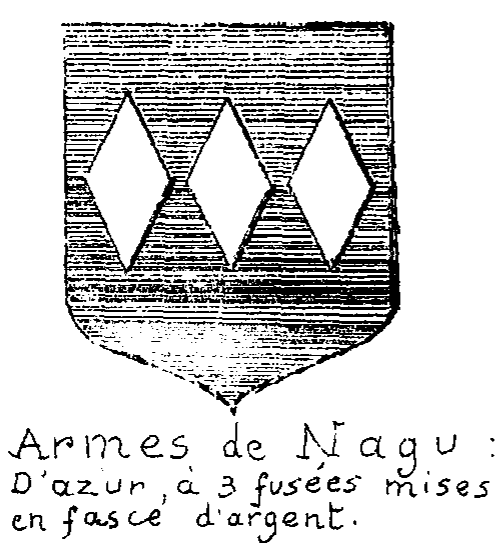
\includegraphics[width=0.50\textwidth]{Illustrations/illus-nagu-armoiries.png}
\end{minipage}\hfill
\begin{minipage}[t]{0.46\textwidth}
    \vspace{-0.5\baselineskip}
    \subsection*{Famille de Nagu}
    La famille de Nagu a appartenu de toute antiquité à la famille du même nom, l'une des plus anciennes et des plus illustres de nos contrées. La filiation suivie que nous possédons de cette famille ne remonte qu'à l'époque où elle quitte Ouroux pour se fixer à Varennes, commune de Quincié en 1374.
\end{minipage}

L'Album Lyonnais nous a conservé le nom de Milon Nagu qui vivait en l'année 1088.

Dans la Charte DCIX du Cartulaire de Mâcon, nous trouvons comme témoin de la vente passée par Guigue, chantre, de tous ses biens situés à Crèches, Jehan de Oratorio. Il est possible que ce témoin fût un des membres de la famille de Nagu. Cet acte solennel fait en faveur de l'église de Mâcon permet de supposer qu'on s'adressa à des hommes occupant un certain rang pour y apposer leur signature. Cette Charte nous reporte aux années comprises dans la période de 1121 à 1143.

Le troisième dont le nom nous soit parvenu est Henri de Nagu.

% --- Page imprimée 40 — vue 43
Il se trouvait à Acre en 1240 et fit par conséquent partie de ces expéditions que les historiens comprennent sous le titre de sixième croisade.

Beaudoin de Courtenay, successeur de Jean de Brienne sur le trône de Constantinople, encouragé et soutenu par le pape Grégoire IX, vint en Occident faire appel au dévouement des chevaliers. Parmi ceux qui écoutèrent sa voix, nous pouvons citer Humbert V, sire de Beaujeu, qui prit part à toutes les guerres religieuses de son siècle. En se rendant en Orient, il passa par Metz ; il data de cette ville la Charte de donation de la dîme d'Ouroux à l'église et aux chanoines de N.D. de Beaujeu pour acquitter la somme de 100 sols léguée à cette église par son frère Louis de Beaujeu (1239)

La même année une nouvelle expédition s'organisa pour aller secourir les Chrétientés de la Terre Sainte sous les ordres de Thibaud, Comte de Champagne. L'un des principaux chefs était Guy IV, Comte de Forez. Henri de Nagu fit partie de ce corps d'armée qui s'embarqua à Marseille et à Aigues-Mortes. Arrivés à Acre, les Croisés firent de cette ville la base de leurs opérations militaires. L'expédition échoua et les Croisés, profondément découragés, reprirent le chemin de l'Occident (1241)

Aucun autre détail ne nous a été conservé sur Henri de Nagu. Comme nous le dirons en parlant de l'église, il est probable qu'à son retour de Terre Sainte, en souvenir de son pèlerinage à Jérusalem, il fit construire la chapelle de Ste-Croix, actuellement de St-Antoine.

Il faut arriver au siècle suivant pour retrouver le nom de Nagu, encore ne s'agit-il point d'un possesseur du fief qui nous occupe ? Nous voyons en effet un Simon de Nagu "prieur de Donseurre ès années 1350 et 1355". Il était probablement oncle de Jean de Nagu, le premier des Seigneurs de Varennes, le dernier qui ait résidé à Ouroux. Ici doit s'arrêter à proprement parler, l'histoire de leur fief. Au départ de la famille de Nagu, il fut morcelé et vendu et si le nom continue de subsister encore dans les siècles suivants il est toujours cité avec ses titres de dépendance.

% --- Page imprimée 41 — vue 44
Jusqu'à ce jour tous les historiens qui se sont occupés du Beaujolais aussi bien que ceux qui ont eu à parler de la famille de Nagu ont avoué qu'il n'existe aucun indice permettant de fixer même approximativement l'époque où le château seigneurial d'Ouroux fut détruit. Monsieur de Lacarelle ; bien à même cependant d'être renseigné, se contenta d'ajouter : "tout porte à croire qu'il aura succombé dans la catastrophe dont on retrouve tant de traces à Ouroux". À quelle époque remonte donc cette catastrophe ? Car il est incontestable qu'à chaque fouille faite dans le bourg on constate la présence de cendres, de débris calcinés, de fers tordus et brûlés.

Il nous paraît certain à cette heure, que nous en devons rechercher la cause dans les incursions que firent dans nos contrées, vers la fin du XIV° siècle, les Routiers et les Tard-Venus. Il n'existe sur cette époque, il est vrai, aucun document écrit qui vienne confirmer nos conclusions ; mais, remarquons-le, il en est de même pour toutes les localités plus importantes que la nôtre. Nous du moins, nous avons une tradition, des preuves matérielles d'une destruction complète du bourg ; les considérations qui vont suivre nous permettront d'en déterminer la date.

C'était pendant la guerre de Cent ans. Jean le Bon avait été fait prisonnier à la funeste bataille de Poitiers (1356). Malgré leur triomphe, les partisans du roi de Navarre et d'Angleterre ne licencièrent pas leurs hommes. Pour eux, la guerre était un métier et la plupart n'avaient d'autre moyen d'existence que le pillage. Ils passèrent en masse sur la terre de France ; plus de trois cent mille de ces vieux soldats aguerris ravagèrent successivement la Bourgogne, le Lyonnais et le Bourbonnais. Dès 1359, ils envahirent le Beaujolais. Antoine, Sire de Beaujeu, ayant fait appel au Comte de Savoie, les rejeta vers le Forez.

Le roi de France, à la suite du traité de Brétigny (1360), était rentré dans son royaume. Les conditions fort onéreuses qui lui furent imposées, l'ordre à rétablir dans ses états, la nécessité de soumettre spécialement dans le Nord, des Seigneurs qui s'étaient rendus indépendants, ne lui permirent pas de secourir immédiatement nos provinces dévastées. De nouvelles bandes de routiers fondirent
% --- Page imprimée 42 — vue 45 (suite)
sur nos montagnes s'emparèrent de Beaujeu et mirent le siège devant le château. Antoine fit de nouveau appel à son allié, le Comte de Savoie et mit de nouveau en fuite les ennemis.

Ne pouvant s'attaquer directement au Château toujours prêt à repousser une surprise, les Tard-Venus se dispersèrent dans les bourgs et les villages,

\begin{wrapfigure}{r}{0.39\textwidth}
    \vspace{-0.4\baselineskip}
    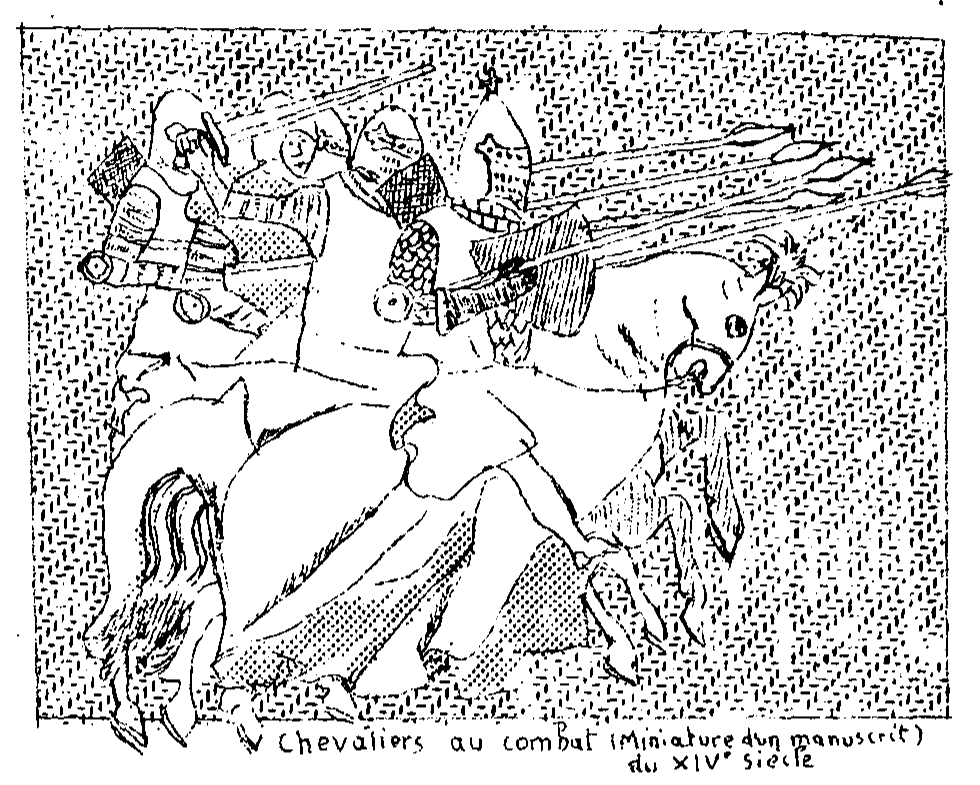
\includegraphics[width=0.36\textwidth]{Illustrations/illus-nagu-chevaliers-combat.png}
\end{wrapfigure}

vivant de pillage, tranquilles au milieu des pays qu'ils infestaient, sûrs qu'ils étaient de l'impunité. La cohésion manquait pour la défense ; chaque ville s'imposait les plus lourds sacrifices pour organiser une résistance le plus souvent inutile, car les ennemis trop bien instruits des préparatifs faits contre eux, se gardaient bien d'affronter la lutte.

Lyon fit appel aux armées du roi qui furent taillées en pièces à la bataille de Brignais le 6 Avril 1362. Ce succès ne fit qu'encourager les Tard-Venus. Le 1er Novembre 1364, leur chef, Seguin de Badefol s'empara d'Anse qui lui servit comme de quartier général pour, de là, rayonner sur les localités environnantes. Les historiens nous disent qu'à ce moment les Grandes Compagnies possédaient plus de soixante maisons fortes dans le Mâconnais, le Forez, le Valais et la Basse-Bourgogne. Sur chaque paroisse du Beaujolais on levait un droit de feuage « pour Messire Seguin de Badefol ».

En 1365, Duguesclin qui se préparait à soutenir les droits de Henri de Transtamare contre son frère Pierre le Cruel sur le trône de Castille les enrôla et les conduisit en Espagne. Enfin trois ans après, la guerre recommençait avec les Anglais, les routiers, rentrés en France, vendant leurs services au plus offrant, s'engagèrent dans les deux armées et s'entredétruisirent les uns les autres.

Treize années de désordres, de pillage et de meurtres durent laisser bien des ruines dans nos contrées. Ouroux, par sa position
% --- Page imprimée 43 — vue 46 (suite)
offrait une proie facile. Alloignet n'existait déjà plus à cette époque comme maison forte et le château de Nagu était le seul point qui put offrir un semblant de résistance aux envahisseurs.

Ils avaient d'ailleurs une vengeance personnelle à satisfaire. Jean de Nagu, l'homme lige du Sire de Beaujeu, était au service d'Antoine, leur plus redoutable adversaire. Ne pouvant réduire à composition le Château de Pierre-Aigüe, il était naturel qu'ils exerçassent des représailles contre les propriétés de ses hommes d'armes. Ouroux fut incendié et son château rasé.

Nous avons parlé plus haut des constructions dont on a retrouvé les traces de chaque côté de la tour de Nagu et que recouvrait une épaisse couche de terre. A 5 mètres de profondeur nous avons pu constater des traces évidentes d'incendie, incendie qui n'a dû rencontrer aucun obstacle, car tout est réduit en cendres ; aucun débris de bois à moitié calciné.

Les ouvriers découvrirent plusieurs médailles que personne n'avait pu classer mais qui, d'après la description donnée par des témoins oculaires, devaient être attribuées, quelques unes du moins, à Amédée de Savoie. Ces médailles, malheureusement, ont été dispersées et il est impossible d'en retrouver la trace.

En 1887, Monsieur GONNET dut procéder à de nouveaux déblaiements dans la même direction que celle des fouilles précédentes, au midi de la tour. Le travail, peu important d'ailleurs, ne pouvait permettre d'espérer de riches découvertes. Celles qui furent faites suffisent néanmoins, semble-t-il, pour permettre de reporter la date de la destruction du château à l'époque des incursions des Grandes Compagnies. Ces médailles sont au nombre de quatre : deux appartiennent à Amédée VIII Comte, puis Duc de Savoie (1391-1439) ; un royal parisis double de Philippe-le-Bel (1285-1314) ; un demi-blanc de Louis XI (1461-1483). Les deux quarts de Gros d'Amédée ont été frappés à des époques différentes : l'un pendant qu'il était Comte, l'autre pendant qu'il était Duc.

Le sol de la construction était recouvert de débris de tuiles et de cendres. Il était facile, après les démolitions des murailles de constater que le terrain coupé en talus était un terrain de
% --- Page imprimée 44 — vue 47 (suite)
transport et qu'il était venu buter contre ces murailles à une époque postérieure à leur construction. Comment expliquer le glissement d'une masse aussi considérable de terre végétale ? Les murs de soutènement qui doivent exister du temps des Seigneurs n'étaient plus entretenus après leur départ aussi bien que l'écroulement des épaisses murailles du château durent en être la véritable cause.

Les monnaies d'Amédée furent découvertes à 0 m 30 au-dessus des cendres. On trouve assez fréquemment même dans le travail le plus superficiel exigé par les jardins, des pièces de monnaies françaises et étrangères, parfois aussi anciennes que celles d'Amédée. Ce fait s'explique naturellement par le passage continuel des troupes dans notre vallée et dont la plupart séjournaient à Ouroux. Mais la présence de celles qui ont été trouvées près de la tour, dans la couche la plus profonde du terrain, ne peut s'expliquer qu'en admettant que ce terrain a dû glisser au plus tôt vers le milieu du XVe siècle, plus tard les documents ou la tradition nous en eussent conservé le souvenir.

Si maintenant nous étudions la généalogie de la famille de NAGU, nous y trouvons une nouvelle confirmation de notre thèse.

Jean de NAGU fut le premier des Seigneur de ce nom qui possédèrent le fief de Varennes ; la disparition des titres qu'il devait posséder à Ouroux avait été si complète que l'auteur de la généalogie des NAGU ne peut citer aucun nom, aucun document concernant cette famille avant 1374. A partir de cette année il a conservé à l'histoire les noms, les dignités, les faits remarquables de chacun de ses membres.

Jean de NAGU avait reçu par testament, en 1374, d'Antoine de Beaujeu mort cette même année, les revenus du fief de Frégny, 500 francs d'or et la Châtellenie de Thizy. Le suzerain voulait ainsi récompenser son fidèle vassal des preuves de dévouement que celui-ci lui avait prodigué dans les guerres incessantes qu'il avait dû soutenir. Devenu possesseur du fief de Varennes en 1395, ne trouvant à Ouroux que des ruines, rien de surprenant qu'il s'empressât de quitter notre vallée pour se rendre à Quincié ! Son fief fut morcelé et
% --- Page imprimée 45 — vue 48 (suite)
vendu ; en ce qui concerne le bourg, une partie passa au Seigneur de Gorze, l'autre à un notaire d'Ouroux du nom de De Bosco.

Le terrier du prieuré de Vauxrenard terminé en 1459 nous offre une indication précieuse. Dans une reconnaissance faite par De Bosco de ses biens mouvant du prieuré, il est dit : « item de bono qui quondam fuit Johannis Nagu… juxta iter per quod itur de Oratorio apud Friaulx » (de même, pour le bien qui fut autrefois de Jean de Nagu… près du chemin qui tend d'Ouroux aux Friats). Mêmes expressions pour la terre de Pollet.

Ces deux reconnaissances nous montrent Jean de Nagu dernier propriétaire des fonds dépendant directement de leur seigneurie d'Ouroux. A partir de cette époque, nous ne trouvons plus aucune trace de possession quelconque à un membre de cette famille dans la partie de la paroisse qui constituait plus particulièrement le fief.

Il nous semble donc permis de conclure que la date de la catastrophe dont la tradition nous a conservé le souvenir doit être reportée à l'époque où les Grandes Compagnies ravagèrent notre province ; Jean de NAGU, enrichi par les largesses du Sire de Beaujeu, renonça à relever son château d'Ouroux et vendit les terres qui en dépendaient.

Le fief de NAGU, avons nous dit, fut morcelé et vendu. De BOSCO fit acquisition de la partie du bourg que posséda plus tard la famille DULIGIER. Un membre de la branche cadette de la famille DE GORZE acheta divers tenements et entr'autres le quartier du bourg traversé par la Grosne. (Nous avons une preuve de ce fait, dans la vente passée par Jean Joseph Berthet de Gorze au profit du Sieur Louis Dubost de Tavane de la maison située au chevet de l'église acquise plus tard par Monsieur GUILLIN pour y installer l'école des filles. Louis Dubost la vendit à son tour à Guillaume Montel écuyer, bourgeois de St-Mamert. Celui-ci céda, par acte passé le 25 Avril 1739, à Claude Monnet de Jullié la somme de 100 livres en principal imposé sur cette maison, moyennant une rente de 5 livres). Celui-ci voulut introduire à Ouroux une industrie nouvelle. Il fit construire dans le pré qui appartient aujourd'hui (en 1890) à la cure, de l'autre côté de la rivière, une tannerie. Cette parcelle de terrain porte encore aujourd'hui le nom « tannerie ».

% --- Page imprimée 46 — vue 49
Les droits seigneuriaux de NAGU furent vendus au possesseur de NAY, fief situé sur la paroisse de Tramayes, au-dessus de la Grosne, au nord-ouest du Clairon.

Philippe de Moles Chantemerle en donnait le dénombrement le 13 Mars 1559. En 1619, la Dame de Vougy, veuve de Claude de Chantemerle cèda à Vincent de Lafond, notaire à Tramayes et l'un des membres de la famille du même nom résident à Ouroux ; les Cens de NAY et NAGU, moyennant la somme de 675 livres.

En 1630, Jacques PALLATIN du DYS, époux de Léonarde Damas, prend le titre de Seigneur de NAY et NAGU ; enfin en 1637, le Baron de LUGNY de la maison de Lévis fut mis en possession de la Seigneurie de NAY par la Comtesse de Montperoux. Aucun document ne nous a permis de découvrir les causes de ces multiples transformations.

Philippe de Moles Chantemerle dont nous venons de parler était seigneur de Vougy, paroisse du Roannais. En 1400, Antoine de Moles avait fait l'aveu de ce fief. Ses enfants Henri et Mérand renouvelèrent cette formalité en 1406. Henri mourut sans enfants vers 1490 et substitua à son nom et à ses armes Philippe de Chantemerle son neveu et son légataire universel.

La famille de GORZE acquit des commissaires du duc de Montpensier la justice de Nagu. Dès le commencement du XVIIe siècle le préambule des divers actes est ainsi conçu : « Par devant nous, Monsieur le Juge ordinaire de Nagu membre dépendant de Nay ou Monsieur son lieutenant… » Il s'agit bien ici du Seigneur de Gorze comme nous le prouve un acte de vente faite en 1679. Jacques Dumont, sieur de l'Etan est juge à cette époque des terres et Seigneuries de Gorze, la Salle, Combe, Nagu et Saccomd pour Philibert Berthet, écuyer seigneur haut justicier desdits lieux ; Ph. Salvay est greffier de la même justice. Quelques années auparavant un membre de la famille De Lafont occupait cette même place.

\begin{figure}[h!]
    \centering
    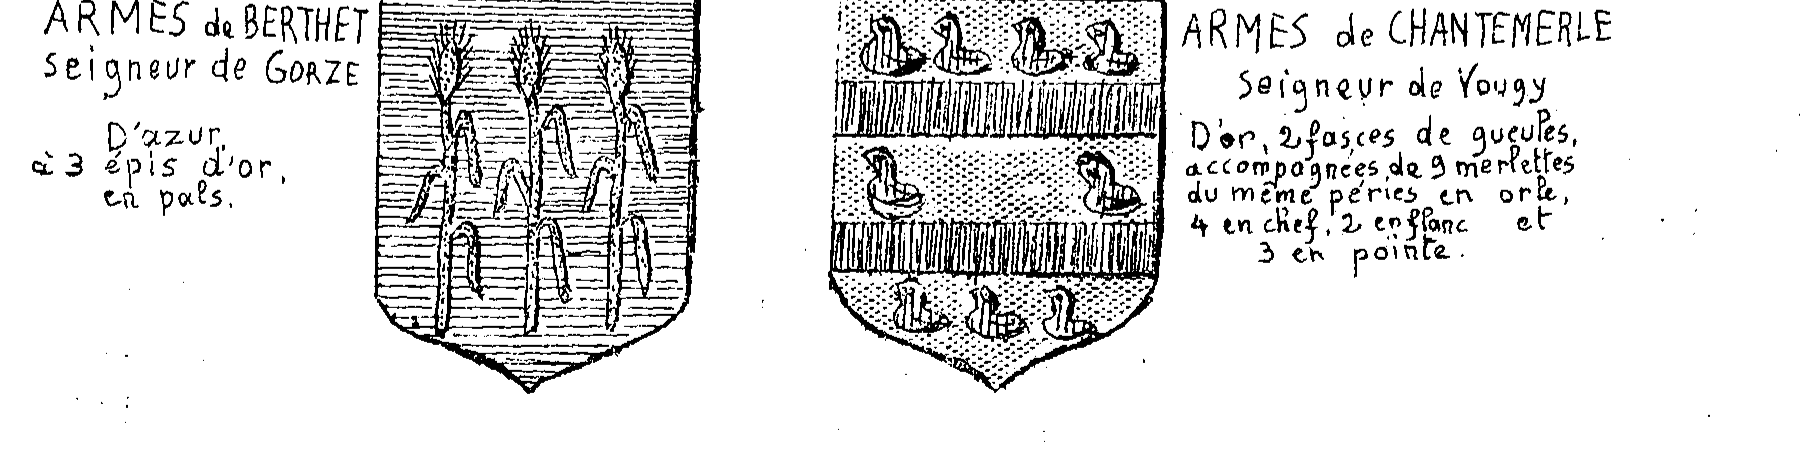
\includegraphics[width=0.78\textwidth]{Illustrations/illus-nagu-armoiries-berthet-chantemerle.png}
\end{figure}
